\documentclass[a4paper,11pt]{article}

%----package----

\usepackage{amsmath}
\usepackage{amssymb}
\usepackage{amsthm}
\usepackage{graphicx}
\usepackage{enumerate}
% Yijia
\usepackage{tikz}
\usepackage{parskip}
\usepackage{hyperref}

%------------------

%\setlength{\topmargin}{0.0in}
%\setlength{\textheight}{10in}
%\setlength{\oddsidemargin}{0.0in}
%\setlength{\evensidemargin}{0.0in}
%\setlength{\textwidth}{6.5in}

%----theorem----
\newtheorem{theorem}{Theorem}[section]
\newtheorem{proposition}[theorem]{Proposition}
\newtheorem{lemma}[theorem]{Lemma}
\newtheorem{corollary}[theorem]{Corollary}
\newtheorem{conjecture}[theorem]{Conjecture}


\theoremstyle{definition}
\newtheorem{definition}[theorem]{Definition}
\newtheorem*{example}{Example}

%----Color----
\definecolor{segment}{HTML}{F4CB70}
\definecolor{remainder}{HTML}{B9DDD8}
\definecolor{undercurve}{HTML}{D7C4EA}
\definecolor{outline}{HTML}{B65C45}
\definecolor{curve}{HTML}{345C91}

%----Command----
\newcommand{\dd}{\mathrm{d}}

%----Body----

\begin{document}
	
\title{The Area of Parabolic Segment}
\author{Yijia Zhao}
\date{\today}
\maketitle

%----------------------------

\section{Problem}

% Condition
A parabolic segment is a region bounded by a parabola and one of its chords. Let $CD$ be such a chord and let $AB$ be a tangent that is parallel to $CD$. Connecting $AD$ and $BC$ which is perpendicular to the $x$-axis to form a parallelogram $ABCD$ shown in Figure~\ref{fig:parabolic-segment}.

We investigate two questions:
\begin{enumerate}
    \item Where does the parabola touch the side $AB$?
    \item How is the area of the parabolic segment related to the area of the parallelogram $ABCD$?
\end{enumerate}

% Figure
\begin{figure}[htbp]
\centering
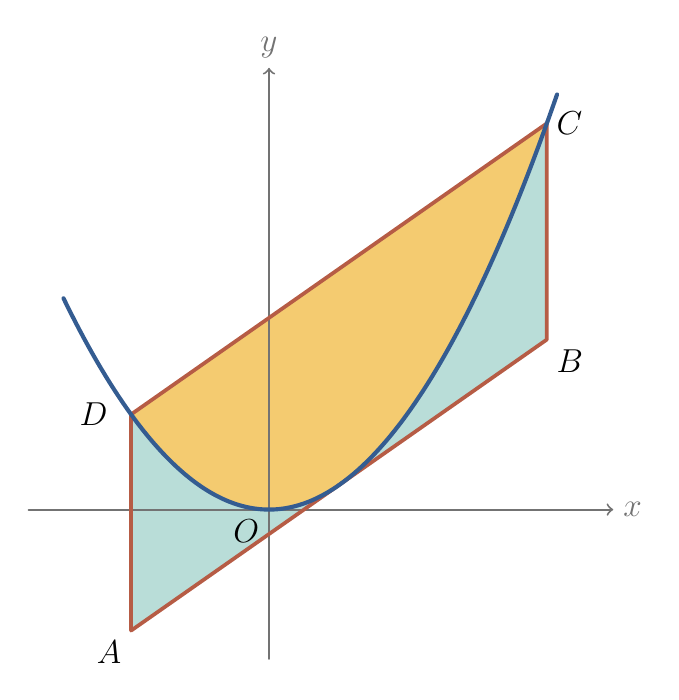
\begin{tikzpicture}[x=1.65cm,y=1.65cm,
  line cap=round,line join=round,font=\large]
  % Translate the original figure by (7/13,49/260).
  \pgfmathsetmacro{\dx}{7/13}
  \pgfmathsetmacro{\dy}{49/260}
  \pgfmathsetmacro{\leftend}{-1.6+\dx}
  \pgfmathsetmacro{\rightend}{1.6+\dx}
  \coordinate (A) at ({-1.6+\dx},{-1.12+\dy});
  \coordinate (B) at ({ 1.6+\dx},{ 1.12+\dy});
  \coordinate (C) at ({ 1.6+\dx},{ 2.784+\dy});
  \coordinate (D) at ({-1.6+\dx},{ 0.544+\dy});

  \fill[remainder] (A)--(B)--(C)--(D)--cycle;
  \fill[segment] (D)--(C)
    --plot[domain=\rightend:\leftend,samples=100]
      (\x,{0.65*\x*\x})--cycle;

  % Coordinate axes; no EF segment or E,F point markers.
  \draw[->,black!55,line width=0.7pt]
    (-1.85,0)--(2.65,0) node[right] {$x$};
  \draw[->,black!55,line width=0.7pt]
    (0,-1.15)--(0,3.4) node[above] {$y$};
  \node[below left] at (0,0) {$O$};

  \draw[outline,line width=1.35pt] (A)--(B)--(C)--(D)--cycle;
  \draw[curve,line width=1.5pt]
    plot[domain={-2.12+\dx}:{1.68+\dx},samples=120]
      (\x,{0.65*\x*\x});
  \node[below left] at (A) {$A$};
  \node[below right] at (B) {$B$};
  \node[right] at (C) {$C$};
  \node[left=5pt] at (D) {$D$};
\end{tikzpicture}
\caption{The parabolic segment bounded by the parabola
and the chord $CD$, inscribed in the parallelogram $ABCD$.}
\label{fig:parabolic-segment}
\end{figure}

%----------------------------

\section{Solution}

% Step 1
Denote the equation of the parabola as $y=ax^2$. We could write the coordinates at $D$ and $C$ as:
$$
D: (x_1, ax_1^2)\;and\;C:(x_2,ax_2^2)
$$
Without loss of generality, we assume $a>0$ and $x_1<x_2$.

% Step 2
First we prove $E$ is the midpoint of $AB$, $|AE|=|EB|$. Shown in Figure~\ref{fig:with-midline}.

% Figure
\begin{figure}[htbp]
    \centering
    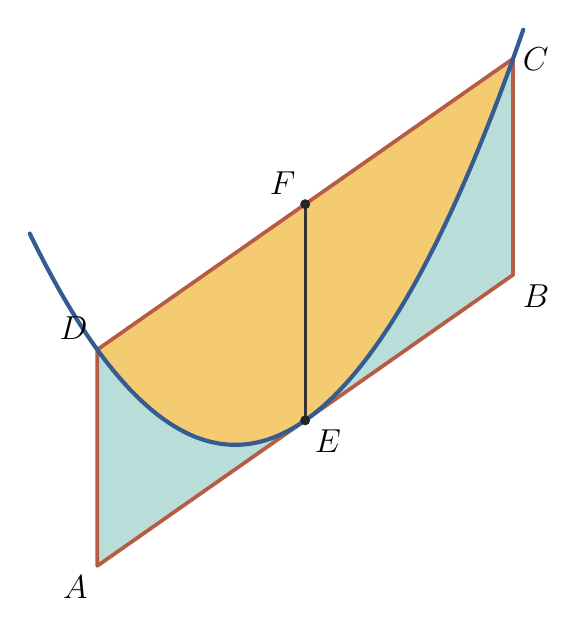
\begin{tikzpicture}[x=1.65cm,y=1.65cm,
      line cap=round,line join=round,font=\large]
      % Parabola: y=0.65*x^2. Its tangent at E has slope 0.7.
      % Translating the construction preserves its original appearance.
      \pgfmathsetmacro{\xe}{0.7/(2*0.65)}
      \pgfmathsetmacro{\ye}{0.65*\xe*\xe}
      \pgfmathsetmacro{\xl}{\xe-1.6}
      \pgfmathsetmacro{\xr}{\xe+1.6}
      \pgfmathsetmacro{\curveleft}{\xe-2.12}
      \pgfmathsetmacro{\curveright}{\xe+1.68}
      \coordinate (A) at (\xl,{\ye-1.12});
      \coordinate (B) at (\xr,{\ye+1.12});
      \coordinate (C) at (\xr,{0.65*\xr*\xr});
      \coordinate (D) at (\xl,{0.65*\xl*\xl});
      \coordinate (E) at (\xe,\ye);
      \coordinate (F) at (\xe,{\ye+1.664});
    
      % Fill the parallelogram, then the parabolic segment.
      \fill[remainder] (A)--(B)--(C)--(D)--cycle;
      \fill[segment] (D)--(C)
        --plot[domain=\xr:\xl,samples=100]
          (\x,{0.65*\x*\x})--cycle;
    
      \draw[outline,line width=1.35pt] (A)--(B)--(C)--(D)--cycle;
      \draw[curve,line width=1.5pt]
        plot[domain=\curveleft:\curveright,samples=120]
          (\x,{0.65*\x*\x});
      \draw[black!80,line width=1.2pt] (E)--(F);
      \foreach \p in {E,F}
        \fill[black!85] (\p) circle[radius=1.8pt];
    
      \node[below left]  at (A) {$A$};
      \node[below right] at (B) {$B$};
      \node[right]       at (C) {$C$};
      \node[above left]  at (D) {$D$};
      \node[below right] at (E) {$E$};
      \node[above left]  at (F) {$F$};
    \end{tikzpicture}
    \caption{$E$ is the point of tangency between the parabola and the tangent line, and $F$ lies on $CD$ such that $EF$ is perpendicular to the $x$-axis.}
    \label{fig:with-midline}
\end{figure}

We consider the gradient of $CD$:
$$
m_{CD}=\frac{ax_2^2-ax_1^2}{x_2-x_1}=a(x_1+x_2)
$$

Denote the $x$-coordinate of $E$ is $x_E$, as $AB$ is a tangent of the parabola, the gradient of $AB$:
$$
m_{AB}=\left.\frac{\dd y}{\dd x}\right|_{x=x_E}=2ax_E
$$

As $AB\parallel CD$, 
$$
m_{AB}=m_{CD} \implies x_E=\frac{x_1+x_2}{2}
$$

$AD$ and $BC$ is perpendicular to the $x$-axis, the $x$-coordinates of $A$ and $B$ are $x_1$, $x_2$ respectively. So $E$ is the midpoint of $AB$.

\newpage

% Step 3
Then we investigate the relationship between area of the parabolic segment and the parallelogram $ABCD$.

As $E$ is also on the parabola, the coordinates of $E$, $(x_E,y_E)$, are: 
$$
\begin{cases}
x_E=\frac{x_1+x_2}{2} \\
y_E=ax_E^2=\frac{a(x_1+x_2)^2}{4}
\end{cases}
$$

Let us consider the coordinates of $F$, $(x_F,y_F)$. As $E$ is the midpoint of $AB$ and $EF\parallel AD$, $F$ is also the midpoint of $CD$ due to the property of parallelogram. So the coordinates of $F$ can be expressed using the midpoint formula:
$$
\begin{cases}
x_F=\frac{x_1+x_2}{2} \\
y_F=\frac{a(x_1^2+x_2^2)}{2}
\end{cases}
$$

Then we can know the length of line $EF$:
$$
|EF|=|y_F-y_E|=\frac{a(x_1^2+x_2^2)}{2}-\frac{a(x_1+x_2)^2}{4}=\frac{a(x_2-x_1)^2}{4}
$$

% Step 4
As $EF\parallel AD$, $AEFD$ is also a parallelogram, $|AD|=|EF|$. We can express the area $A_p$ of parallelogram $ABCD$:
$$
A_p=|AD||x_C-x_D|=|EF||x_2-x_1|=\frac{a(x_2-x_1)^3}{4}
$$

% Step 5
Next, let us find the area of parabolic segment by calculus. Let $G$ be the where $AD$ meet $x$-axis and let $H$ be the point where the extended $CB$ meet $x$-axis shown in Figure~\ref{fig:with-calculus}.

The area $A_i$, bounded by the parabola, $DG$, $CH$ and $x$-axis(purple part in Figure~\ref{fig:with-calculus}) equals to:
$$
A_i=\int_{x_1}^{x_2} ax^2dx=\left.\frac{ax^3}{3}\right|_{x=x_1}^{x=x_2}=\frac{a(x_2^3-x_1^3)}{3}
$$

% Step 6
The area, $A_t$, of trapezium $CDGH$ can also be expressed:
$$
A_t=\frac{1}{2}(|DG|+|CH|)|GH|=\frac{a(x_1^2+x_2^2)}{2}(x_2-x_1)
$$
and the area $A_s$ of parabolic segment (yellow part in Figure~\ref{fig:with-calculus}) equals to:
$$
A_s=A_t-A_i=\frac{a(x_1^2+x_2^2)}{2}(x_2-x_1)-\frac{a(x_2^3-x_1^3)}{3}=\frac{a(x_2-x_1)^3}{6}
$$

\newpage

% Step 8
Finally, the relationship between the area of the parabolic segment($A_s$), and the area of parallelogram $ABCD$($A_p$) is:
$$
\frac{A_s}{A_p}=\frac{a(x_2-x_1)^3}{6}\div\frac{a(x_2-x_1)^3}{4}=\frac{2}{3}
$$

% Figure
\begin{figure}[htbp]
    \centering
    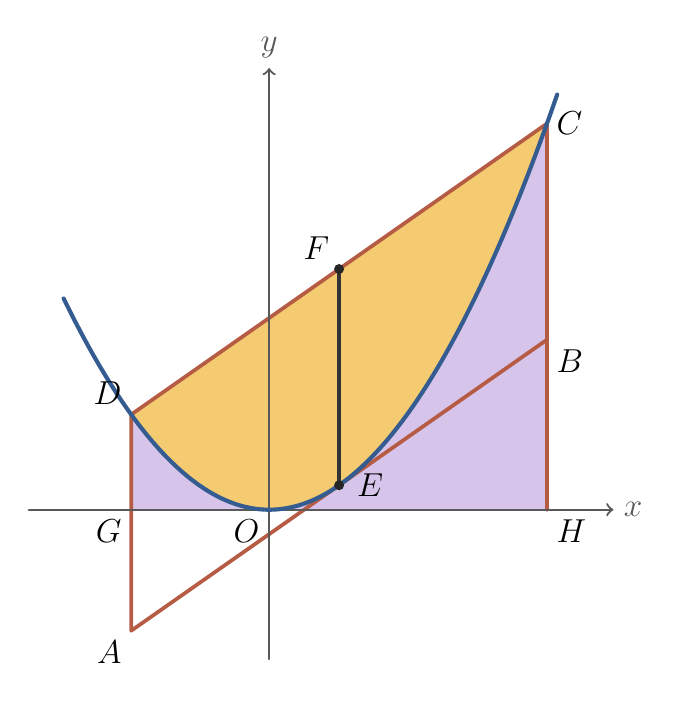
\begin{tikzpicture}[x=1.65cm,y=1.65cm,
      line cap=round,line join=round,font=\large]
      % Parabola: y=0.65*x^2. Its tangent at E has slope 0.7.
      \pgfmathsetmacro{\xe}{0.7/(2*0.65)}
      \pgfmathsetmacro{\ye}{0.65*\xe*\xe}
      \pgfmathsetmacro{\xl}{\xe-1.6}
      \pgfmathsetmacro{\xr}{\xe+1.6}
      \pgfmathsetmacro{\curveleft}{\xe-2.12}
      \pgfmathsetmacro{\curveright}{\xe+1.68}
      \coordinate (A) at (\xl,{\ye-1.12});
      \coordinate (B) at (\xr,{\ye+1.12});
      \coordinate (C) at (\xr,{0.65*\xr*\xr});
      \coordinate (D) at (\xl,{0.65*\xl*\xl});
      \coordinate (E) at (\xe,\ye);
      \coordinate (F) at (\xe,{\ye+1.664});
      \coordinate (G) at (\xl,0);
      \coordinate (H) at (\xr,0);
    
      % Area under the parabola between the vertical lines AD and CB.
      \fill[undercurve] (G)--(H)--(C)
        --plot[domain=\xr:\xl,samples=100]
          (\x,{0.65*\x*\x})--cycle;
      % Keep the original parabolic segment above the curve.
      \fill[segment] (D)--(C)
        --plot[domain=\xr:\xl,samples=100]
          (\x,{0.65*\x*\x})--cycle;
    
      \draw[outline,line width=1.35pt] (A)--(B)--(C)--(D)--cycle;
      \draw[outline,line width=1.35pt] (B)--(H);
      \draw[->,black!65,line width=0.8pt]
        (-1.85,0)--(2.65,0) node[right] {$x$};
      \draw[->,black!65,line width=0.8pt]
        (0,-1.15)--(0,3.4) node[above] {$y$};
      \node[below left] at (0,0) {$O$};
      \draw[curve,line width=1.5pt]
        plot[domain=\curveleft:\curveright,samples=120]
          (\x,{0.65*\x*\x});
      \draw[black!80,line width=1.2pt] (E)--(F);
      \foreach \p in {E,F}
        \fill[black!85] (\p) circle[radius=1.8pt];
    
      \node[below left]  at (A) {$A$};
      \node[below right] at (B) {$B$};
      \node[right]       at (C) {$C$};
      \node[above left]  at (D) {$D$};
      \node[right,xshift=3pt] at (E) {$E$};
      \node[above left]  at (F) {$F$};
      \node[below left]  at (G) {$G$};
      \node[below right] at (H) {$H$};
    \end{tikzpicture}
    \caption{The purple region shows the area under the parabola between $G$ and $H$ on the $x$-axis.}
    \label{fig:with-calculus}
\end{figure}
\hfill$\square$

% Use of AI
\section*{Declaration of AI use}
The TikZ code used to produce the figures in this document
was generated using OpenAI Codex (GPT-6.1 Sol). The code was reviewed by the author.

% Code
\section*{Source code}
The LaTeX source code for this document is available at:
\url{https://github.com/Yijia-phys/mathematical-inverstigation/mini-project-parabolic-segment/}

\end{document}
